% nt-05-genealogy.tex

\documentclass[xcolor=dvipsnames]{beamer}
\usepackage{teachbeamer}

\title{Nietzsche and Genealogy}
\subtitle{{\CourseNumber}, {\CourseInst}}

\author{\CourseName}

\date{June 14, 2018}

\begin{document}

\begin{frame}
  \titlepage
\end{frame}

% \begin{frame}
%   \frametitle{iClicker Question}
% Choose from the following options. This item will be graded.
% \begin{block}{iClicker Question}
% [6595] Which geological epoch plays a special role in Bernard Williams' chapter about genealogy?
% \end{block}
% \begin{description}
% \item[A\hspace{.2in}$\blacktriangleright$] the pliocene
% \item[B\hspace{.2in}$\blacktriangleright$] the paleocene
% \item[C\hspace{.2in}$\blacktriangleright$] the pleistocene
% \item[D\hspace{.2in}$\blacktriangleright$] the holocene
% \end{description}
% \end{frame}

% \begin{frame}
%   \frametitle{iClicker Question}
% Choose from the following options. This item will be graded.
% \begin{block}{iClicker Question}
% [7252] What kind of story does Bernard Williams investigate in order to write a genealogy of truthfulness?
% \end{block}
% \begin{description}
% \item[A\hspace{.2in}$\blacktriangleright$] a children's story
% \item[B\hspace{.2in}$\blacktriangleright$] a literary story
% \item[C\hspace{.2in}$\blacktriangleright$] a state of nature story
% \item[D\hspace{.2in}$\blacktriangleright$] an autobiography
% \end{description}
% \end{frame}

% \begin{frame}
%   \frametitle{iClicker Question}
% Choose from the following options. This item will be graded.
% \begin{block}{iClicker Question}
% [1976] Which of these stories (genealogies) does Raymond Geuss tell in detail?
% \end{block}
% \begin{description}
% \item[A\hspace{.2in}$\blacktriangleright$] Modern Physics (via Planck and Einstein)
% \item[B\hspace{.2in}$\blacktriangleright$] Enlightenment (via Kant and Hume)
% \item[C\hspace{.2in}$\blacktriangleright$] Judaism (via Moses and Abraham)
% \item[D\hspace{.2in}$\blacktriangleright$] Christianity (via Paul and Jesus)
% \end{description}
% \end{frame}

% \begin{frame}
%   \frametitle{iClicker Question}
% Choose from the following options. This item will be graded.
% \begin{block}{iClicker Question}
% [3977] Raymond Geuss contrasts providing a genealogy with {\ldots}
% \end{block}
% \begin{description}
% \item[A\hspace{.2in}$\blacktriangleright$] {\ldots} giving a pedigree
% \item[B\hspace{.2in}$\blacktriangleright$] {\ldots} writing an autobiography
% \item[C\hspace{.2in}$\blacktriangleright$] {\ldots} compiling computer code
% \item[D\hspace{.2in}$\blacktriangleright$] {\ldots} composing a symphony
% \end{description}
% \end{frame}

\begin{frame}
  \frametitle{Truth and Truthfulness}
  Traditional theories of truth:
  \begin{enumerate}
  \item Correspondence Theory (what makes a belief true is its
    correspondence to a state in the world)
  \item Coherence Theory (what makes a belief true is the coherence of
    the belief system of which it is a part)
  \item Pragmatist Theory (truth is the end of inquiry; truth is
    satisfactory to believe)
  \end{enumerate}
  You may be a realist or an anti-realist (Michael Dummett) about
  truth. Deflationists about truth think that there is no metaphysical
  substance in the truth predicate because the proposition X and the
  proposition ``X is true'' are equivalent.
\end{frame}

\begin{frame}
  \frametitle{Geuss' View on Nietzsche and Truth}
  \begin{block}{Raymond Geuss: Nietzsche and Genealogy}
    If Nietzsche clearly attacks the correspondence view, shows no
    interest in coherence, and seems to present no clear alternative
    of his own invention, then he must tacitly hold some kind of
    reductivist or pragmatist view [according to Habermas]. The most
    fruitful way of taking Nietzsche seems to me to see him not as
    trying to propound his own variant theory of truth, but as
    formulating a new question ``How and why does the will-to-truth
    come about?'' (and claiming that this question is more interesting
    than, and doesn't presuppose an antecedent answer to Plato's
    question ``What is truth?''). (8)
  \end{block}
\end{frame}

\begin{frame}
  \frametitle{Truth and Truthfulness}
  It is difficult to keep the things that Nietzsche says about truth
  consistent. On the one hand, Williams lauds his attachment to the
  truth in so far as Nietzsche resists the cowardice of believing
  errors. On the other hand, Nietzsche is famously dismissive of
  objective and metaphysical truth.

  \bigskip

  Williams appears to be distinguishing between an attitude of
  \alert{truthfulness}, which is willing to believe something that is
  not useful or happymaking; and \alert{truth}, about whose origins
  there may be a genealogy.
  \begin{block}{Friedrich Nietzsche, The Gay Science, 167}
    We should not reinterpret the exceedingly derivative, late, rare,
    accidental, that we perceive only on the crust of the earth and
    make of it something essential, universal, and eternal. 
  \end{block}
\end{frame}

\begin{frame}
  \frametitle{Truth and Truthfulness}
  Key points about Nietzsche's attitude towards truth.
  \begin{itemize}
  \item ``fundamental insight: there is no pre-established harmony
    between the furthering of truth and the well-being of humanity''
    (does Nietzsche's view of truth square with his will to power
    monism?)
  \item ``it is still a metaphysical faith upon which our faith in
    science rests''
  \item ``error is not blindness---error is cowardice''
  \item nothing is really identical, all identity is a fiction (17)
  \item ``the antithesis of the apparent world and the true world is
    reduced to the antithesis world and nothing''
  \end{itemize}
\end{frame}

\begin{frame}
  \frametitle{Masking}
  \begin{block}{Michel Foucault: Histoire de la sexualit{\'e},
      page 113}
    C'est {\`a} la condition de masquer une part importante de
    lui-m{\^e}me que le pouvoir est tol{\'e}rable. Sa r{\'e}ussite
    est en proportion de ce qu'il parvient {\`a} cacher de ses
    m{\'e}canismes. Le pouvoir serait-it accept{\'e} s'il
    {\'e}tait enti{\`e}rement cynique? Le secret n'est pas pour
    lui de l'ordre de l'abus: il est indispensable {\`a} son
    fonctionnement.
  \end{block}
\end{frame}

\begin{frame}
  \frametitle{Genealogy I}
  \begin{block}{Bernard Williams: Truth and Truthfulness, 28}
  A genealogy is a narrative that tries to explain a cultural
  phenomenon by describing a way in which it came about {\ldots} Our
  ethical ideas are a complex deposit of many different traditions and
  social forces, and they have themselves been shaped by
  self-conscious representations of that history. However, the impact
  of these historical processes is to some extent concealed by the
  ways in which their product thinks of itself.
  \end{block}
\end{frame}

\begin{frame}
  \frametitle{Genealogy II}
  \begin{block}{Michel Foucault: Nietzsche, Genealogy, History, 142}
    However, if the genealogist refuses to extend his faith in
    metaphysics, if he listens to history, he finds that there is
    ``something altogether different'' behind things: not a timeless and
    essential secret, but the secrets that they have no essence or
    that their essence was fabricated in a piecemeal fashion from
    alien forms.
  \end{block}
\end{frame}

\begin{frame}
  \frametitle{Genealogy III}
    In the context of Hume's account of moral responsibility,
    genealogy denotes the kind of explanation pointing to the origins
    of a social practice of which it is essential that they themselves
    are not used as reasons to follow the practice. The core of the
    practice is somehow constituted by a certain forgetfulness toward
    its history. The forgetfulness is at the root of lending the
    practice intrinsic rather than instrumental value: a value which
    becomes detached from the original usefulness of the practice;
    also a value which experiences a threat to its reflective
    stability, and possibly a breakdown, when its historical origins
    are uncovered.
\end{frame}

\begin{frame}
  \frametitle{Genealogy IV}
Here are some examples for cultural phenomena (it may be very
controversial whether these really are cultural phenomena!) that have
been submitted to genealogies:
\begin{enumerate}
\item truth (Friedrich Nietzsche)
\item justice (David Hume)
\item morality (Friedrich Nietzsche)
\item gender (Judith Butler)
\item knowledge (Michel Foucault, Archaeology of Knowledge)
\item love (the prairie vole)
\item soul (Michel Foucault, The Body of the Condemned)
\end{enumerate}
\end{frame}

\begin{frame}
  \frametitle{Prairie Voles and Montane Voles}
  \begin{itemize}
  \item Prairie voles mate for life, and montane voles do not.
  \item Among prairie voles, the males not only share parenting
    duties, they will even lick and nurture pups that aren't their
    own.
  \item By contrast, male montane voles do not actively parent even
    their own offspring.
  \end{itemize}
  What accounts for the difference? Researchers have found that the
  prairie voles have greater numbers of oxytocin receptors in certain
  regions of the brain. Prairie voles that have had their oxytocin
  receptors blocked will not pair-bond. An object lesson in
  neuro-philosophy?
\end{frame}

\begin{frame}
  \frametitle{State of Nature Stories}
State of nature stories operate on simplified, imaginary environments.
  \begin{itemize}
  \item justice (D. Hume)
  \item state (R. Nozick)
  \item knowledge (E.J. Craig)
  \item truth (B. Williams)
  \item morality? (F. Nietzsche)
  \end{itemize}
  The state of nature is not the pleistocene. What characterizes
  humans naturalistically is their massive potential for non-genetic learning.
\end{frame}

\begin{frame}
  \frametitle{Just-So Stories}
  In 1902, Rudyard Kipling published a book called \emph{Just So
    Stories}. The term was appropriated in a derogatory fashion to
  discredit various types of evolutionary hypothesis about adaptation.
  The problem is usually that the hypothesis comes without means of
  empirical falsification.

  \bigskip

  \begin{tabular}{|c|c|c|}\hline
    & sons & daughters \\ \hline
    general-status mother & 2.8 & 1.7 \\ \hline
    low-status mother & 2.3 & 2.6 \\ \hline
  \end{tabular}

  \bigskip

  Trivers-Willard hypothesis. Williams makes the point that just-so
  stories may be fact-defective, but that doesn't automatically make
  them law-defective.
\end{frame}

\begin{frame}
  \frametitle{Function and Explanation}
  A property (such as altruism or other collaborative dispositions)
  may function to make individuals and the societies in which they
  live more fit. Williams correctly points out that functional
  accounts are not explanations. They lack historical plausibility
  since rational deliberation about the value of a property in the
  development of this property would beg the question. The prisoner
  dilemma illustrates this problem formally.

  \bigskip

  One way in which evolutionary psychology may overcome this problem
  is by introducing intrinsic (versus instrumental) goals. A parent
  does not come to the aid of a child because the well-being of the
  child is of instrumental value (in order to promote the gene
  propagation of near kin); the well-being of the child is of
  intrinsic value. This leads to a genealogy, which may either be
  vindicatory (Nozick: state) or non-vindicatory (Nietzsche:
  morality). 
\end{frame}

\begin{frame}
  \frametitle{Truth and Truthfulness}
  Williams' genealogy of truthfulness turns out to be vindicatory, and
  it entails that correspondence to facts is of intrinsic value.
  \begin{description}
  \item[truth] metaphysical, not historical
  \item[sincerity] historical, instrumental
  \item[truthfulness] historical, intrinsic
  \end{description}
\end{frame}

\begin{frame}
  \frametitle{Salvator Mundi: Pedigree or Genealogy}
      \begin{figure}[h]
    \includegraphics[scale=.33]{./davinci_salvator-mundi_grt.jpg}
  \end{figure}
\end{frame}

\begin{frame}
  \frametitle{Salvator Mundi: Pedigree or Genealogy}
  \begin{enumerate}
  \item Louis XII of France (around 1500)
  \item Henrietta Maria (wife of Charles I of England, around 1625)
  \item John Stone (1651, for perhaps as little as 30 pounds)
  \item returned to Charles II of England (English Restoration, 1660)
  \item {\ldots} (third wives, illegitimate children, etc.) {\ldots}
  \item George III (1763)
  \item {\ldots} painting disappears {\ldots}
  \item Francis Cook (1900)
  \item sold for 45 pounds in 1958, painting disappears again
  \item Robert Simon purchases the painting for \$10,000 in 2005 at an
    auction in New Orleans
  \item Swiss dealer Yves Bouvier purchases the painting for
    \$75,000,000 in 2013
  \item Dmitry Rybolovlev immediately purchases the painting for
    \$127,500,000
  \item Mohammed bin Salman purchases the painting for \$450,312,500
    in 2017
  \end{enumerate}
\end{frame}

\begin{frame}
  \frametitle{Pedigree and Genealogy}
  These are characteristic features of a pedigree, to be contrasted
  with a genealogy according to Raymond Geuss.
  \begin{itemize}
  \item positive valorization
  \item linearity
  \item singular origin
  \end{itemize}
\end{frame}

\begin{frame}
  \frametitle{Genealogy of Christianity}
  As opposed to a pedigree of Christianity, in a genealogy of
  Christianity there 
  \begin{itemize}
  \item are diverse lines of development (a synthesis)
  \item is a migration of concepts (the debtor-creditor relationship)
  \item is a history ``doused in blood'' (i.e.\ violent and oppressive)
  \item are contingencies (breaks, leaps, and coercions, GM II, 17)
  \item are individuals (Paul) and collectives (the Church, the
    mendicants) who impress their interpretation on a tradition
    (Foucault makes collective wills more precise with his theory of
    microdominations)
  \item self-contradictions that lead to eventual demise (compare
    Marx' dialectical materialism)
  \end{itemize}
\end{frame}

\begin{frame}
  \frametitle{Beware of Avant-Guard Dog}
  \begin{figure}[h]
    \includegraphics[scale=0.28]{./BewareTheAvantGuardDog.jpg}
  \end{figure}
\end{frame}

\begin{frame}
  \frametitle{Structuralism Table}
\begin{figure}[h]
\includegraphics[scale=.3]{./structable.png}
\end{figure}
\end{frame}

\begin{frame}
  \frametitle{Nietzsche, Genealogy, History}
  These are the errors that, with Nietzsche's help, Foucault
  identifies about Paul R{\'e}e's historical explanation of morality:
  \begin{itemize}
  \item linear development
  \item exclusive concern for utility (Mill's utility monism)
  \item semiotic stability (words, desires, ideas keep their meaning/direction/logic)
  \end{itemize}
  Paul R{\'e}e ``ignored the fact that the world of speech and desires
  has known invasions, struggles, plundering, disguises, ploys'' (139).
\end{frame}

\begin{frame}
  \frametitle{Nietzsche, Genealogy, History}
  Genealogy
  \begin{itemize}
  \item demands relentless erudition
  \item rejects the metahistorical deployment of ideal significations
    and indefinite teleologies (140)
  \end{itemize}
  Pursuit of the origin (Ursprung)
  \begin{itemize}
  \item attempts to capture the exact essence of things, their purest
    possibilities, and their carefully protected identities (142)
  \item assumes the existence of immobile forms that precede the
    external world of accident and succession
  \item is a search for primordial truth
  \end{itemize}
\end{frame}

\begin{frame}
  \frametitle{Nietzsche, Genealogy, History}
  ``Liberty is an `invention of the ruling classes' and fundamental to
  man's nature or at the root of his attachment to being and truth''
  (142). Disparity is at the historical origin. Foucault on
  narrative coherence:
  \begin{quote}
    Where the soul pretends unification or the self fabricates a
    coherent identity, the genealogist sets out to study the
    beginning---numberless beginnings, whose faint traces and hints of
    colour are readily seen by a historical eye. The analysis of
    descent permits the dissociation of the self, its recognition and
    displacement as an empty synthesis, in liberating a profusion of
    lost events. (145f)
  \end{quote}
\end{frame}

\begin{frame}
  \frametitle{Microdominations}
  In ``Nietzsche, Genealogy, History,'' Foucault calls it the
  ``endlessly repeated play of dominations.'' It 
  \begin{itemize}
  \item leads to the differentiation of values
  \item leads to the idea of liberty (macrodominations on a class level)
  \item established marks of its power and engraves memories on things
    and even within bodies (the ``inscription on a body,'' see Kafka's
    ``Penal Colony'')
  \end{itemize}
\end{frame}

\begin{frame}
  \frametitle{The Role of the Law}
  The law is not opposed to violence (contra Hobbes), but the law is a
  ``calculated and relentless pleasure, delight in the promised
  blood'' (151).
  \begin{quote}
    The desire for peace, the serenity of compromise, and the tacit
    acceptance of the law, far from representing a major moral
    conversion or a utilitarian calculation that gave rise to the law,
    are but its result and, in point of fact, its perversion: ``guilt,
    conscience, and duty had their threshold of emergence in the right
    to secure obligations; and their inception, like that of any major
    event on earth, was saturated in blood.'' Humanity does not
    gradually progress from combat to combat until it arrives at
    universal reciprocity, where the rule of law finally replaces
    warfare; humanity installs each of its violences in a system of
    rules and thus proceeds from domination to domination. (151)
  \end{quote}
\end{frame}

\begin{frame}
  \frametitle{Two Accounts of Interpretation}
  \begin{quote}
    If interpretation were the slow exposure of the meaning hidden in
    an origin, then only metaphysics could interpret the development
    of humanity. But if interpretation is the violent or surreptitious
    appropriation of a system of rules, which in itself has no
    essential meaning, in order to impose a direction, to bend it to a
    new will, to force its participation in a different game, and to
    subject it to secondary rules, then the development of humanity is
    a series of interpretations.
  \end{quote}
\end{frame}

\begin{frame}
  \frametitle{Traditional vs. Effective History}
  \begin{tabular}{|l|l|}\hline
    \textbf{traditional} & \textbf{effective} \\ \hline
    historical constants & no historical constants \\ \hline
    consoling play of recognitions & multiplying the body \\ \hline
    rediscovery & discontinuity \\ \hline
    knowledge made for cutting & knowledge made for cutting \\ \hline
    find regulative mechanisms & find most unique characteristics \\ \hline
    primordial intention & singular randomness \\ \hline
    essential traits and final meanings & profusion of entangled events \\ \hline
    kinship to philosophy & kinship to medicine \\ \hline
    objectivity & perspective \\ \hline
  \end{tabular}
\end{frame}

\begin{frame}
  \frametitle{Three Platonic Modalities}
  Effective history frees the historical sense from the demands of a
  suprahistorical history.

  \bigskip

  \begin{tabular}{rcl}
    parody & vs. & reality \\
    dissociation & vs. & identity \\
    sacrifice & vs. & truth \\
  \end{tabular}
\end{frame}

\begin{frame}
  \frametitle{Foucault and Authenticity}
  \begin{quote}
    He will not be too serious to enjoy it; on the contrary, he will
    push the masquerade to its limit and prepare the great carnival of
    time where masks are constantly reappearing {\ldots} taking up
    these masks, revitalizing the buffoonery of history, we adopt an
    identity whose unreality surpasses that of God, who started the
    charade. (161)
  \end{quote}
  Antiquarian history ``seeks the continuities of soil, language, and
  urban life in which our present is rooted, and, `by cultivating in a
  delicate manner that which existed for all time, it tries to
  conserve for posterity the conditions under which we were born'\,''
  (162).
\end{frame}

\begin{frame}
  \frametitle{Hermeneutics of Trust}
  For Gadamer, a hermeneutics of suspicion is always derivative of a
  hermeneutics of trust (the contrast between the two is due to Paul
  Ricoeur, who wrote about this after Gadamer published \emph{Truth
    and Method}). Gadamer says, ``only when this assumption proves
  mistaken [the assumption that the text has integrity]---i.e.\ the
  text is not intelligible---do we begin to suspect the text'' (294).
  Understanding is like speaking your native language: it is natural,
  constitutive of being. Misunderstanding is derivative and
  artificial, such as when someone speaks to you in a foreign language
  that you do not understand.
  \begin{quote}
    It is only when the attempt to accept what is said as true fails
    that we try to ``understand'' the text, psychologically or
    historically, as another's opinion (294)
  \end{quote}
\end{frame}

\begin{frame}
  \frametitle{Paul Ricoeur's Hermeneutics of Trust/Suspicion}
  \alert{Hermeneutics of the sacred} (Bultmann, Gadamer), where
  demythologizing is not meant to discredit symbols, but to recover
  original meaning. \alert{Hermeneutics of suspicion}, which is not
  concerned with recovering the object, but with tearing away masks,
  with disclosing disguises, with revealing false consciousness.
  \begin{itemize}
  \item Nietzsche: narrative is the masking of will-to-power
  \item Marx: see Antonio Gramsci's theory of cultural hegemony
  \item Freud: narratives are often misleading signals of a rich
    subconscious life (amnesia of ontogenesis)
  \end{itemize}
\end{frame}

\begin{frame}
  \frametitle{Foucault: Two Kinds of Suspicion}
  Michel Foucault starts out his paper ``Nietzsche, Freud, Marx'' with
  two kinds of suspicion towards language:
  \begin{description}
  \item[hyponoia] language does not say what it means
  \item[semainon] there are many other things in the world that speak and that are not language
  \end{description}
\end{frame}

\begin{frame}
  \frametitle{Stages of Interpretation}
  \begin{enumerate}
  \item Corpus of resemblance. Something wants to be said and can be
    deciphered. Deucalion and Pyrrha. 
  \end{enumerate}
\end{frame}

\begin{frame}
  \frametitle{Pyrrha and Deucalion I}
      \begin{figure}[h]
    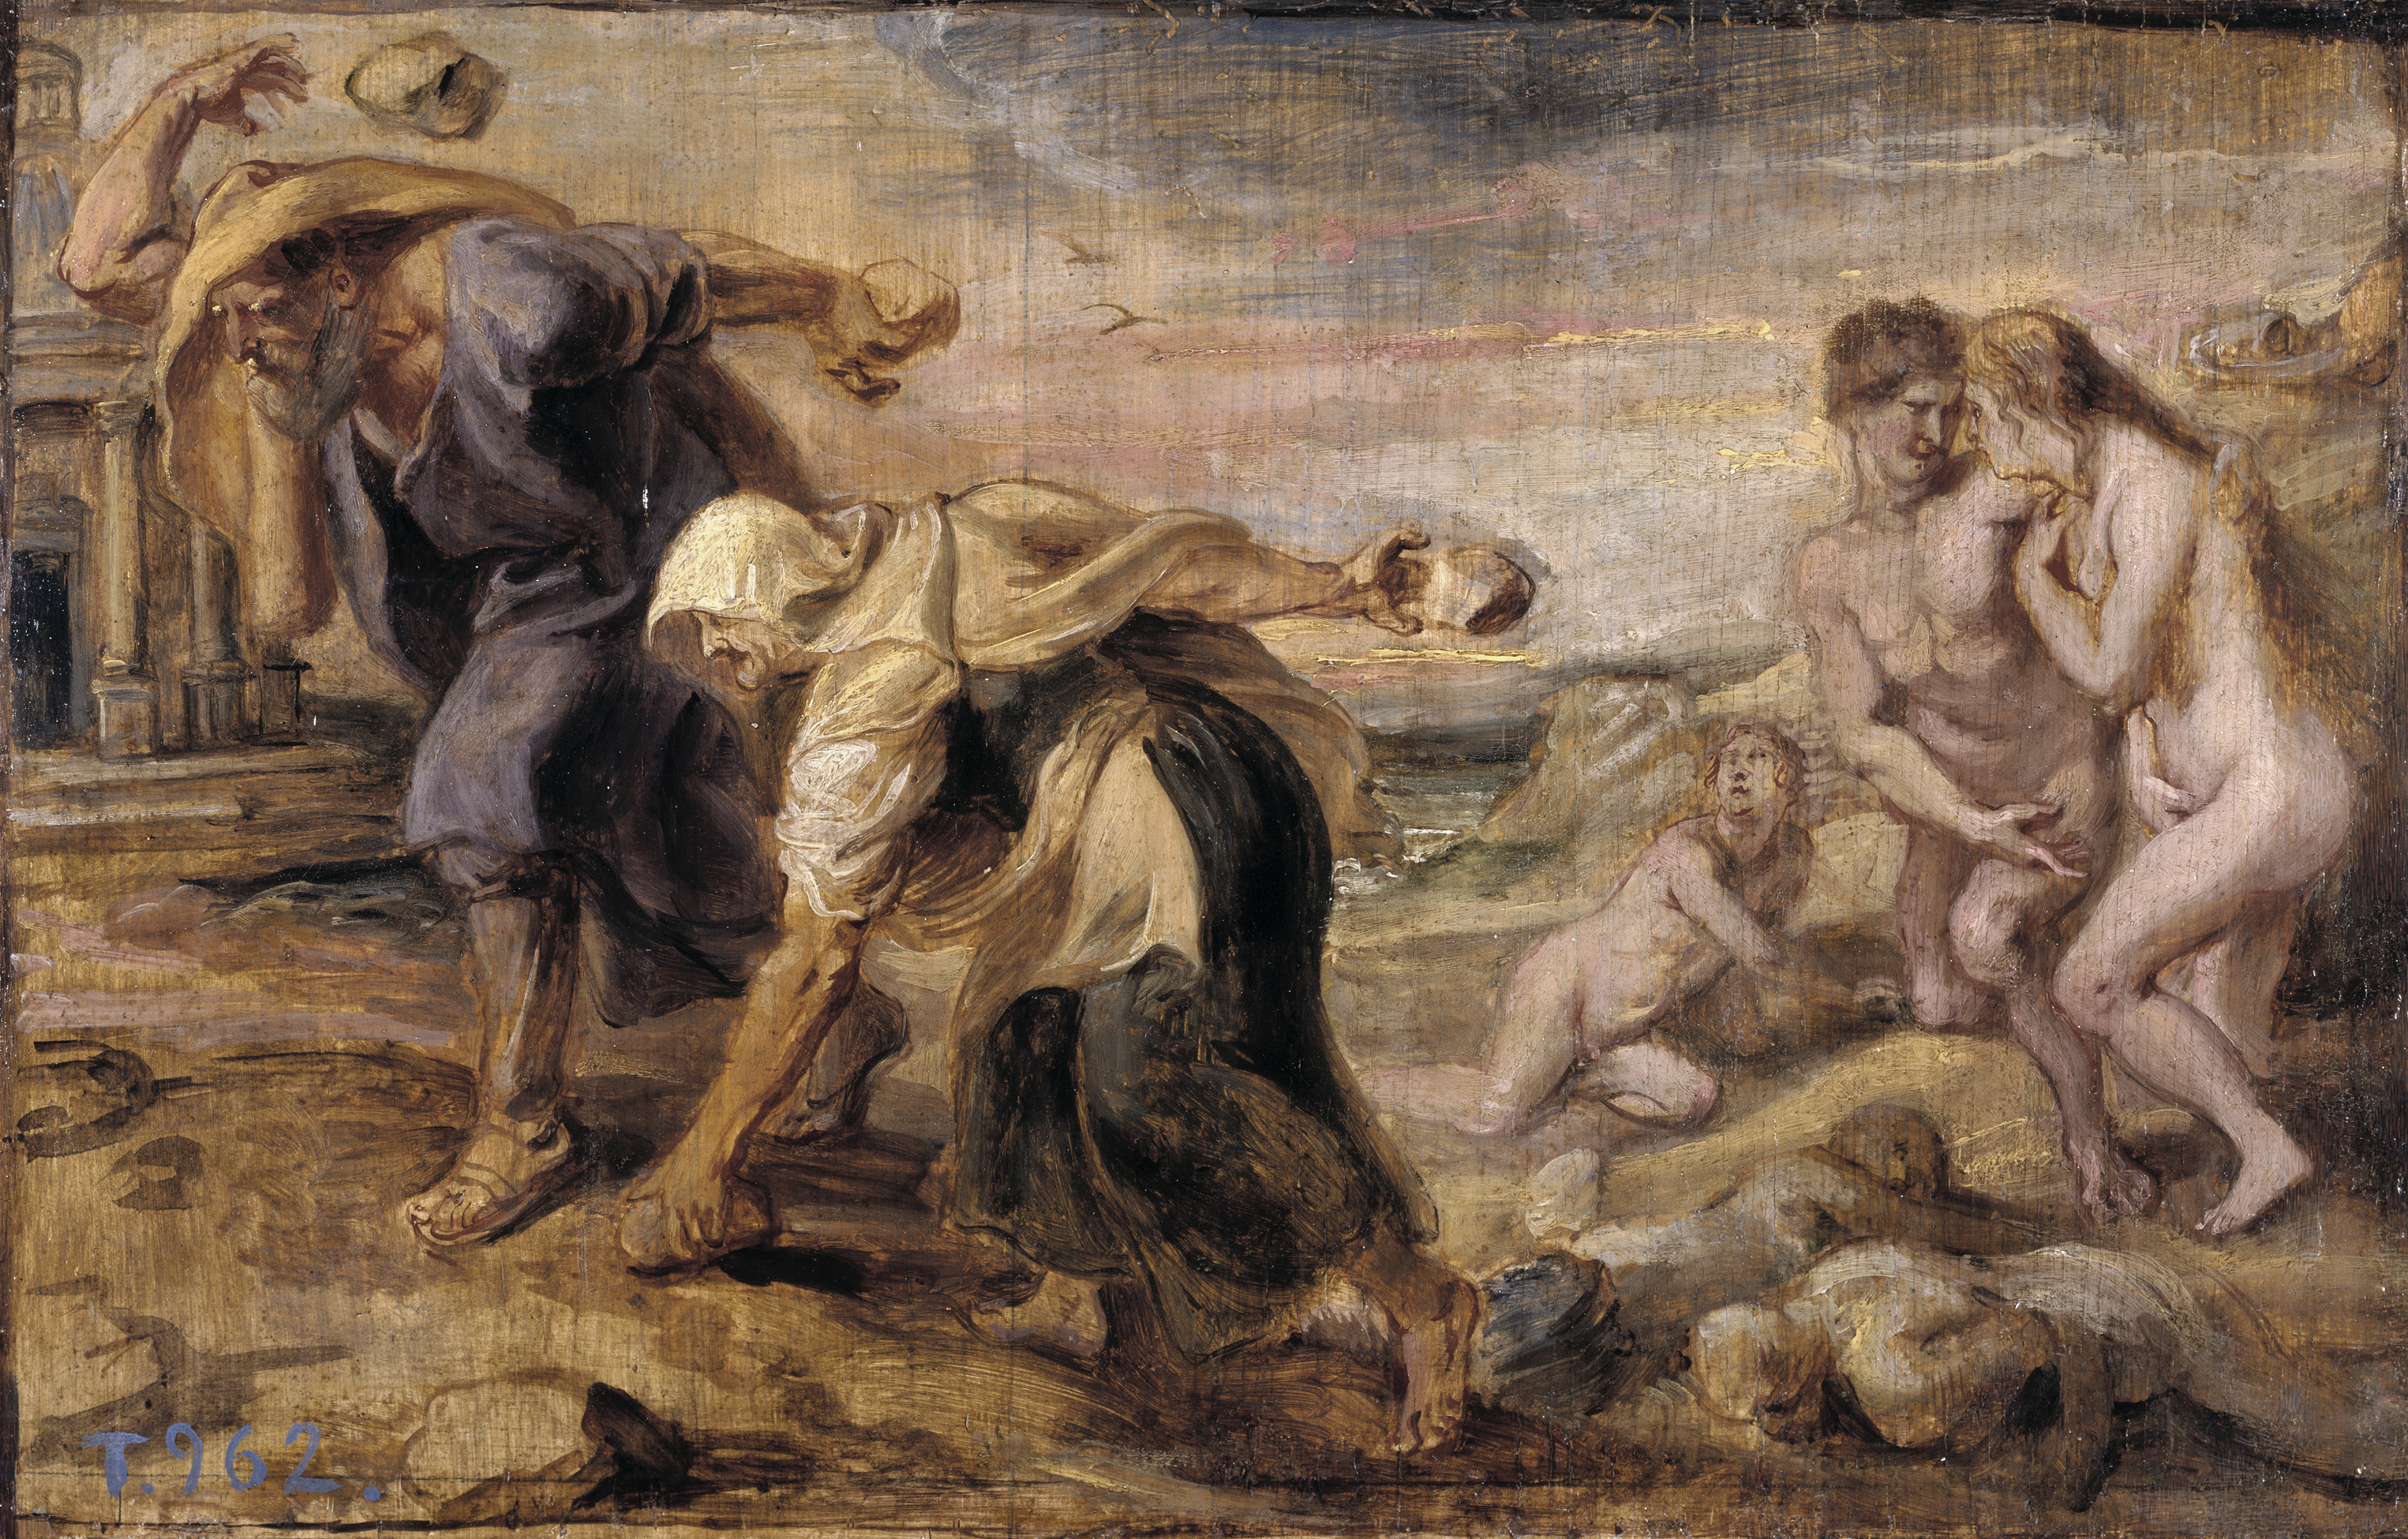
\includegraphics[scale=.47]{./deucalion.jpg}
  \end{figure}
\end{frame}

\begin{frame}
  \frametitle{Pyrrha and Deucalion II}
  When Zeus decided to end the Bronze Age with the great deluge,
  Deucalion and his wife, Pyrrha, were the only survivors. Even though
  he was imprisoned, Prometheus who could see the future and had
  foreseen the coming of this flood told his son, Deucalion, to build
  an ark and, thus, they survived. During the flood, they landed on
  Mount Parnassus, the only place spared by the flood.
\end{frame}

\begin{frame}
  \frametitle{Pyrrha and Deucalion III}
  Once the deluge was over and the couple were on land again,
  Deucalion consulted an oracle of Themis about how to repopulate the
  earth. He was told to throw the bones of his mother behind his
  shoulder. Deucalion and Pyrrha understood the ``mother'' to be Gaia,
  the mother of all living things, and the ``bones'' to be rocks. They
  threw the rocks behind their shoulders, which soon began to lose
  their hardness and change form. Their mass grew greater, and the
  beginnings of human form emerged. The parts that were soft and moist
  became skin, the veins of the rock became people's veins, and the
  hardest parts of the rocks became bones. The stones thrown by Pyrrha
  became women; those thrown by Deucalion became men.
\end{frame}

\begin{frame}
  \frametitle{Foucault: History of the Present}
Four general rules:
\begin{enumerate}
\item The concept under consideration fulfills a \alert{complex
    social function}
\item The concept under consideration is specific in the more
  general field of exercising power -- it is a \alert{political
    tactic}
\item the \alert{technology of power} is the principle both of
  humanization and knowledge of man
\item the body invested with power relations \alert{creates the soul}
\end{enumerate}
\end{frame}

\begin{frame}
  \frametitle{The Penal System: A Historical Discontinuity}
  \begin{equation}
    \label{eq:zeiqueex}
    \begin{array}{rcl}
      \mbox{executioner} & \mbox{vs.} & \mbox{army of technicians} \\
      \mbox{punishment of body} & \mbox{vs.} & \mbox{suspension of rights} \\
      \mbox{individual (King and Condemned)} & \mbox{vs.} & \mbox{institution} \\
      \mbox{violence} & \mbox{vs.} & \mbox{bio-power} \\
      \mbox{theatre} & \mbox{vs.} & \mbox{order and silence (7)} \\
      \mbox{law and its subjects} & \mbox{vs.} & \mbox{norms and their subjects} \\
      \mbox{everyday perception} & \mbox{vs.} & \mbox{abstract consciousness (9)} \\
      \mbox{transcendental responsibility} & \mbox{vs.} & \mbox{responsibility relieved by} \\
      \mbox{} & \mbox{} & \mbox{bureaucratic concealment (9)} \\
      \mbox{body as immediate object} & \mbox{vs.} & \mbox{body as intermediate object} \\
      \mbox{punishing the body} & \mbox{vs.} & \mbox{curing the soul} \\
    \end{array}\notag
  \end{equation}
\end{frame}

\begin{frame}
  \frametitle{Foucault: Bio-Power}
  \begin{itemize}
  \item the industrial system requires cheap, efficient labour
    (25)
  \item it is always the body that is at issue -- the body and its
    forces, their utility and their docility, their distribution
    and their submission (25)
  \item there is a knowledge of the body which is not a science of
    its functioning (26)
  \item this knowledge and this mastery constitute the political
    technology of the body (26)
  \item micro-physics of power (26)
  \item the irreducible entanglement of knowledge and power (27)
  \item subjugating human bodies by making them objects of
    knowledge (28) (see \emph{Notes from the Underground})
  \end{itemize}
\end{frame}

\begin{frame}
  \frametitle{Subjectivity}
  \begin{itemize}
  \item ``the psychologists and the minor civil servants of moral
    orthopaedics'' (10), ``army of technicians'' (11), ``there swarms
    a whole series of subsidiary authorities'' (21)
  \item economy of suspended rights
  \item the body as intermediary to the juridical subject
  \item the soul: ``a new character came on the scene, masked'' (16f,
    much more on page 29)
  \item substitution of objects: from crimes to passions, instincts,
    anomalies, infirmities, maladjustments, environmental and
    hereditary effects (when a child is punished, it is now for moral,
    not for practical reasons)
  \item the field of knowledge susceptible of scientific knowledge
    (the textification of the world, if all you have is a hammer,
    everything looks like a nail)
  \item the ``assessing, diagnostic, prognostic, normative judgment''
    (19)
  \end{itemize}
\end{frame}

\begin{frame}
  \frametitle{Dispositif}
  \begin{block}{Michel Foucault}
    {\ldots} one may map {\ldots} through this displacement, a whole
    field of recent objects, a whole new system of truth and a mass of
    roles hitherto unknown in the exercise of criminal justice. A
    corpus of knowledge, techniques, scientific discourses is formed
    and becomes entangled with the practice of the power to punish.
    (23)
  \end{block}
\end{frame}

\begin{frame}
  \frametitle{Marxism and Its Failure}
  \begin{quote}
    The political investment of the body is bound up {\ldots} with its
    economic use; it is largely as a force of production that the body
    is invested with relations of power and domination (26)
  \end{quote}
  \begin{quote}
    What the apparatuses and institutions operate is, in a sense, a
    micro-physics of power {\ldots} this power is exercised rather
    than possessed; it is not the privilege, acquired or preserved, of
    the dominant class, but the overall effect of its strategic
    positions {\ldots} these relations are not localized in the
    relations between the state and its citizens or on the frontier
    between classes (27)
  \end{quote}
\end{frame}

\begin{frame}
  \frametitle{Knowledge}
  \begin{quote}
    Perhaps, too, we should abandon a whole tradition that allows us
    to imagine that knowledge can exist only where the power relations
    are suspended and that knowledge can develop only outside its
    injunctions, its demands, and its interests. Perhaps we should
    abandon the belief that power makes people mad and that, by the
    same token, the renunciation of power is one of the conditions of
    knowledge. We should admit, rather, that power produces knowledge
    (and not simply by encouraging it because it serves power or by
    applying it because it is useful); that power and knowledge
    directly imply one another; that there is no power relation
    without the correlative constitution of a field of knowledge, nor
    any knowledge that does not presuppose and constitute at the same
    time power relations. 
  \end{quote}
\end{frame}

\begin{frame}
  \frametitle{Knowledge}
  \begin{quote}
    These ``power-knowledge relations'' are to be analyzed, therefore,
    not on the basis of a subject of knowledge who is or is not free
    in relation to the power system; but, on the contrary, the subject
    who knows, the objects to be known, and the modalities of
    knowledge must be regarded as so many effects of these fundamental
    implications of power-knowledge and their historical
    transformations. In short, it is not the activity of the subject
    of knowledge that produces a corpus of knowledge, useful or
    resistant to power, but power-knowledge, the processes and
    struggles that traverse it and of which it is made up, that
    determines the forms and possible domains of knowledge. (27f)
  \end{quote}
\end{frame}

\begin{frame}
  \frametitle{The Soul}
  \begin{itemize}
  \item genealogy of the modern soul (29)
  \item the soul is not an illusion, ``it exists, it has a reality, it
    is produced permanently around, on, within the body''
  \item not born in sin and subject to punishment, but born out of
    methods of punishment, supervision, and constraint (the university
    precedes the student)
  \item on it are built scientific techniques and discourses, and the
    moral claims of humanism (30)
  \item the soul (which we long to be free) is the effect and
    instrument of a political anatomy; the soul is the prison of the
    body
  \end{itemize}
\end{frame}

\begin{frame}
  \frametitle{The Soul: An Extended Quote}
  \begin{block}{Michel Foucault: The Body of the Condemned, 29f}
    The history of this micro-physics of the punitive power would the
    be a genealogy or an element in a genealogy of the modern soul.
    Rather than seeing the soul as the reactivated remnants of an
    ideology, one would see it as the present correlative of a certain
    technology of power over the body. 
  \end{block}
\end{frame}

\begin{frame}
  \frametitle{The Soul: An Extended Quote}
  \begin{block}{Michel Foucault: The Body of the Condemned, 29f}
    It would be wrong to say that the soul is an illusion, or an
    ideological effect. On the contrary, it exists, it has a reality,
    it is produced permanently around, on, within the body by the
    functioning of a power that is exercised on those punished---and,
    in a more general way, on those one supervisors, trains and
    corrects, over madmen, children at home and at school, the
    colonized, over those who are stuck at a machine and supervised
    for the rest of their lives.
  \end{block}
\end{frame}

\begin{frame}
  \frametitle{The Soul: An Extended Quote}
  \begin{block}{Michel Foucault: The Body of the Condemned, 29f}
    This is the historical reality of this soul, which, unlike the
    soul represented by Christian theology, is not born in sin and
    subject to punishment, but is born rather out of methods of
    punishment, supervision and constraint. This real, non-corporal
    soul is not a substance; it is the element in which are
    articulated the effects of a certain type of power and the
    reference of a certain type of knowledge, the machinery by which
    the power relations give rise to a possible corpus of knowledge,
    and knowledge extends and reinforces the effects of this power.
  \end{block}
\end{frame}

\begin{frame}
  \frametitle{The Soul: An Extended Quote}
  \begin{block}{Michel Foucault: The Body of the Condemned, 29f}
    On this reality-reference, various concepts have been constructed
    and domains of analysis carved out: psyche, subjectivity,
    personality, consciousness, etc.; on it have been built scientific
    techniques and discourses, and the moral claims of humanism. But
    let there be no misunderstanding: it is not that a real man, the
    object of knowledge, philosophical reflection or technical
    intervention, has been substituted for the soul, the illusion of
    the theologians.
  \end{block}
\end{frame}

\begin{frame}
  \frametitle{The Soul: An Extended Quote}
  \begin{block}{Michel Foucault: The Body of the Condemned, 29f}
    The man described for us, whom we are invited to free, is already
    in himself the effect of a subjection much more profound than
    himself. A soul inhabits him and brings him to existence, which is
    itself a factor in the mastery that power exercises over the body.
    The soul is the effect and instrument of a political anatomy; the
    soul is the prison of the body.
  \end{block}
\end{frame}

\begin{frame}
  \frametitle{Hermeneutics of Sex}
  Here are some ways in which Foucault informs a hermeneutics of sex.
  \begin{itemize}
  \item institutionalized knowledge and power bring sex within the
    purview of hermeneutics
  \item in line with anti-narrativism and the scientific tradition,
    the hegemony of hermeneutics is perceived as a threat
  \item Foucault, however, has no narrative-free alternative (bodies
    inconsequential bucolic pleasures?) to the deployment of
    discourse: interpretation (power/knowledge) creates subjectivity
  \item consequently, Habermas' concept of the ideal speech situation
    is illusory; there is no speech without power (concatenation of
    microdominations)
  \end{itemize}
\end{frame}

\begin{frame}
  \frametitle{Transformation from Feudal to Bourgeois}
  \begin{itemize}
  \item calling sex by its name more costly
  \item discursive explosion based on secrecy
  \item authorized vocabulary
  \item steady proliferation of discourses concerned with sex (18)
  \item an institutional incitement to speak about it
  \item the Christian pastoral
  \item rules of self-examination
  \item the imperative and nearly infinite task to tell (authenticity)
  \item transforming desire into discourse (narrativization of sex)
  \end{itemize}
\end{frame}

\begin{frame}
  \frametitle{Victorianism}
  \begin{itemize}
  \item the author of \emph{My Secret Life} and the halfwit of the
    Lorraine (where bucolic pleasures turn into judicial action,
    medical intervention, clinical examination, and theoretical
    elaboration, 31)
  \item ``the strangest of these practices was the fact of recounting
    them all'' (22, this wouldn't be strange to a narrativist like
    Schechtman or Taylor, for whom the experience must be articulated
    before it can be meaningful)
  \item the convergence of morality and rationality (24, Freud and Pence)
  \end{itemize}
\end{frame}

\begin{frame}
  \frametitle{Bio-Power}
  \begin{itemize}
  \item the emergence of population: birth and death rates, life
    expectancy, fertility, state of health, frequency of illnesses,
    diet, habitation
  \item schools: architectural layout---the question of sex was a
    constant preoccupation (27); the sex of the schoolboy became a
    public problem
  \end{itemize}
\end{frame}

\begin{frame}
  \frametitle{Incitement to Discourse}
  \begin{quote}
    Sex was driven out of hiding and constrained to lead a discursive
    existence. From the singular imperialism that compels everyone to
    transform their sexuality into a perpetual discourse, to the
    manifold mechanisms which, in the areas of economy, pedagogy,
    medicine, and justice, incite, extract, distribute, and
    institutionalize the sexual discourse, an immense verbosity is
    what our civilization has required and organized {\ldots} we talk
    about sex more than anything else {\ldots} we have never said
    enough on the subject {\ldots} speaking of it ad infinitum, while
    exploiting it as the secret
  \end{quote}
\end{frame}

\begin{frame}
  \frametitle{An Observation by Foucault, Introducing Butler}
  In ``Nietzsche, Genealogy, History,'' Foucault writes
  \begin{quote}
    We believe, in any event, that the body obeys the exclusive laws
    of physiology and that it escapes the influence of history, but
    this too is false. The body is molded by a great many distinct
    regimes; it is broken down by the rhythms of work, rest, and
    holidays; it is poisoned by food or values, through eating habits
    or moral laws; it constructs resistances. (153)
  \end{quote}
\end{frame}

\begin{frame}
  \frametitle{The Possibilities of Inversion}
  Consider the following inversions.
  \begin{description}
  \item[Foucault] It is not the subject that determines social power,
    but social power that determines the subject.
  \item[Butler] Sexual identity does not follow from personal
    identity, but personal identity follows from sexual identity.
  \item[Rousseau] The literal meaning does not precede the figurative
    meaning, but the figurative meaning precedes the literal meaning.
  \item[Derrida] Writing, because it is supplemental, intermediate,
    distancing, characterized by transference, the sign of a sign, is
    not the worse, but the better representation of the function of
    language.
  \end{description}
\end{frame}

\begin{frame}
  \frametitle{Sexual Identity}
  Features of the traditional view of identity:
  \begin{itemize}
  \item persisting through time
  \item as the same, unified, and internally coherent
  \item related to consciousness
  \item capacity for language and
  \item moral deliberation
  \end{itemize}
Butler now asks:
\begin{quote}
  To what extent do regulatory practices of gender formation and
  division constitute identity, the internal coherence of the subject?
  (23)
\end{quote}
\end{frame}

\begin{frame}
  \frametitle{Butler Inversions}
  \begin{itemize}
  \item personal identity $\longleftarrow$ gender identity
  \item becoming a person $\longleftarrow$ becoming gendered
  \item identity $\longleftarrow$ regulatory practices
  \item the descriptive $\longleftarrow$ the normative
  \item the doer $\longleftarrow$ the deed
  \end{itemize}
\end{frame}

\begin{frame}
  \frametitle{Intelligible Gender vs Spectres}
  Intelligible genders are those which institute coherence and
  continuity among sex, gender, sexual practice, and desire. They are
  met by the spectres (Marx, ``A specter is haunting Europe'' in the
  \emph{Communist Manifesto}) of discontinuity and incoherence (23).
  They cannot `exist,' because their practices of desire do not follow
  from either sex or gender. The matrix of intelligibility produces
  rival and subversive matrices of gender disorder.
\end{frame}

\begin{frame}
  \frametitle{The Matrix of Intelligibility}
  Identity is an effect of discursive practices (Habermas!). 
  \begin{itemize}
  \item compulsory heterosexuality
  \item totalizing frame
  \item phallogocentrism (the precursor of compulsory heterosexuality)
  \end{itemize}
\end{frame}

\begin{frame}
  \frametitle{Three Views on Gender}
  \begin{description}
  \item[Luce Irigaray] Irigaray is a Belgian philosopher who claims
    that there is only one sex, the masculine, which elaborates itself
    in and through the production of the Other.
  \item[Michel Foucault] The category of sex, whether masculine or
    feminine, is a production of a diffuse regulatory economy of
    sexuality.
  \item[Monique Wittig] Wittig was a French philosopher who claims
    that the category of sex is always feminine because the masculine
    remains unmarked as the universal.
  \end{description}
\end{frame}

\begin{frame}
  \frametitle{The Hermeneutics of Sex}
  \begin{quote}
    Irigaray's theory of sexual preference suggests that women can
    never be understood on the model of a ``subject'' within the
    conventional representational systems of  Western culture
    precisely because they constitute the fetish of representation
    and, hence, the unrepresentable as such. Women can never ``be,''
    according to this ontology of substances, precisely because they
    are the relation of difference, the excluded, by which that domain
    marks itself off. Women are neither the subject nor its Other, but
    a difference from the economy of binary opposition, itself a ruse
    for a monologic elaboration of the masculine. (25)
  \end{quote}
\end{frame}

\begin{frame}
  \frametitle{The Hermeneutics of Sex}
  The grammar of gender masks the univocal and hegemonic discourse of
  the masculine, because being a sex or a gender is fundamentally
  impossible (not if you are an essentialist). For Foucault, the
  binary regulation of sexuality suppresses the subversive
  multiplicity of a sexuality that disrupts heterosexual,
  reproductive, and medicojuridical hegemonies (26).
\end{frame}

\begin{frame}
  \frametitle{Metaphysics of Substance}
The metaphysics of substance, a term associated with Nietzsche, shows
that a number of philosophical ontologies have been trapped within
certain illusions of ``Being'' and ``Substance.'' In no sense,
however, do they reveal or represent some true order of things (28).
Metaphysical substance is often derived from grammar, as in Descartes
``I think therefore I am.''  
\end{frame}

\begin{frame}
  \frametitle{Sexual Desire}
  The matrix of intelligibility is held together by asymmetries of
  sexual desire. There is another inversion here: sexual desire does
  not proceed from sexual identity, but it constitutes it. Sex is not
  the cause for the effects of sexual experience, behaviour, and
  desire; the cause-effect relationship is reversed (Foucault, 32).
  Foucault's antidote: Herculine Barbin, whose experience is ``a world
  of pleasures in which grins hang about without the cat.''
\end{frame}

\begin{frame}
  \frametitle{The Cheshire Cat}
  \begin{figure}[h]
    \includegraphics[scale=0.45]{./cheshire.jpg}
  \end{figure}
\end{frame}

\begin{frame}
  \frametitle{The Cheshire Cat}
  \begin{quote}
    Smiles, happinesses, pleasures, and desires are figured here as
    qualities without an abiding substance to which they are said to
    adhere. As free-floating attributes, they suggest the possibility
    of a gendered experience that cannot be grasped through the
    substantializing and hierarchizing grammar of nouns and
    adjectives. Through his cursory reading of Herculine, Foucault
    proposes an ontology of accidental attributes that exposes the
    postulation of identity as a culturally restricted principle of
    order and hierarchy, a regulatory fiction. (33)
  \end{quote}
\end{frame}

\begin{frame}
  \frametitle{Butler's Claim}
  Butler disagrees with Foucault. Gender is not a noun, but is also
  not a set of free-floating attributes. Gender is performatively
  produced; it is always a doing. The doer is merely a fiction added
  to the deed, as in Descartes-Nietzsche.
\end{frame}

% \begin{frame}
%   \frametitle{iClicker Question}
% Choose from the following options. This item will be graded.
% \begin{block}{iClicker Question}
% [1231] Which relationship develops on the basis of promisekeeping in Nietzsche's genealogy of morality?
% \end{block}
% \begin{description}
% \item[A\hspace{.2in}$\blacktriangleright$] oligarch-plutocrat
% \item[B\hspace{.2in}$\blacktriangleright$] infantry-cavalry
% \item[C\hspace{.2in}$\blacktriangleright$] debtor-creditor
% \item[D\hspace{.2in}$\blacktriangleright$] matrix-meretrix
% \end{description}
% \end{frame}

% \begin{frame}
%   \frametitle{iClicker Question}
% Choose from the following options. This item will be graded.
% \begin{block}{iClicker Question}
% [6033] Fill in the blank: ``if a doctor had treated a {\ldots} for serious internal inflammations which would drive the European with the stoutest constitution to distraction; -- the do \emph{not} do that to the {\ldots}''
% \end{block}
% \begin{description}
% \item[A\hspace{.2in}$\blacktriangleright$] Eskimo
% \item[B\hspace{.2in}$\blacktriangleright$] Muscovite
% \item[C\hspace{.2in}$\blacktriangleright$] Negro
% \item[D\hspace{.2in}$\blacktriangleright$] Extraterrestrial
% \end{description}
% \end{frame}

% \begin{frame}
%   \frametitle{iClicker Question}
% Choose from the following options. This item will be graded.
% \begin{block}{iClicker Question}
% [1507] Which words does Foucault use to illuminate the concept of genealogy?
% \end{block}
% \begin{description}
% \item[A\hspace{.2in}$\blacktriangleright$] gen{\`e}se, origine, provenance
% \item[B\hspace{.2in}$\blacktriangleright$] originem, formatio, cunabula
% \item[C\hspace{.2in}$\blacktriangleright$] diathesis, syntaxis, katastasis
% \item[D\hspace{.2in}$\blacktriangleright$] Ursprung, Entstehung, Herkunft
% \end{description}
% \end{frame}

% \begin{frame}
%   \frametitle{iClicker Question}
% Choose from the following options. This item will be graded.
% \begin{block}{iClicker Question}
% [4256] In Foucault's paper ``Nietzsche, Genealogy, History,'' what kind of history is in contrast to traditional history?
% \end{block}
% \begin{description}
% \item[A\hspace{.2in}$\blacktriangleright$] Gender history
% \item[B\hspace{.2in}$\blacktriangleright$] effective history
% \item[C\hspace{.2in}$\blacktriangleright$] poststructural history
% \item[D\hspace{.2in}$\blacktriangleright$] Marxist history
% \end{description}
% \end{frame}

\begin{frame}
  \frametitle{iClicker Question}
Choose from the following options. This item will be graded.
\begin{block}{iClicker Question}
[6542] What does Foucault identify as a problem with modern discourse about sex?
\end{block}
\begin{description}
\item[A\hspace{.2in}$\blacktriangleright$] modernity is too
  body-focused (instead of mind-focused) in its sexuality
\item[B\hspace{.2in}$\blacktriangleright$] we talk about sexual desire too much
  (the endless mill of speech)
\item[C\hspace{.2in}$\blacktriangleright$] we don't talk about sex
  enough (repressed sexual desire must be articulated)
\item[D\hspace{.2in}$\blacktriangleright$] men want sex, women want
  conversation (gender imbalance with respect to verbal and sexual
  intimacy)
\end{description}
\end{frame}


\begin{frame}
  \frametitle{iClicker Question}
Choose from the following options. This item will be graded.
\begin{block}{iClicker Question}
[6039] What is the narrative eighty years after Damiens' execution to which
the public execution is set in contrast?
\end{block}
\begin{description}
\item[A\hspace{.2in}$\blacktriangleright$] the overcrowding of prisons
\item[B\hspace{.2in}$\blacktriangleright$] the abolition of the death penalty
\item[C\hspace{.2in}$\blacktriangleright$] a timetable of rules for young prisoners
\item[D\hspace{.2in}$\blacktriangleright$] institutional racism in prisons
\end{description}
\end{frame}


\begin{frame}
  \frametitle{iClicker Question}
Choose from the following options. This item will be graded.
\begin{block}{iClicker Question}
[7517] According to Foucault, modern discourse about sex is intimately linked to
\end{block}
\begin{description}
\item[A\hspace{.2in}$\blacktriangleright$] the economic and political problem of population
\item[B\hspace{.2in}$\blacktriangleright$] the fear of sexually-transmitted disease
\item[C\hspace{.2in}$\blacktriangleright$] an erosion of monogamy due to homosexuality
\item[D\hspace{.2in}$\blacktriangleright$] the Christian dogma of the Trinity
\end{description}
\end{frame}


\begin{frame}
  \frametitle{iClicker Question}
Choose from the following options. This item will be graded.
\begin{block}{iClicker Question}
[8509] What, according to Foucault, is the relationship between knowledge and power?
\end{block}
\begin{description}
\item[A\hspace{.2in}$\blacktriangleright$] knowledge and power have separate domains
\item[B\hspace{.2in}$\blacktriangleright$] power corrupts knowledge
\item[C\hspace{.2in}$\blacktriangleright$] power produces knowledge, power and knowledge imply one another
\item[D\hspace{.2in}$\blacktriangleright$] knowledge constrains power
\end{description}
\end{frame}


\begin{frame}
  \frametitle{iClicker Question}
Choose from the following options. This item will be graded.
\begin{block}{iClicker Question}
[9851]   Who is Herculine Barbin (Foucault uses her to show that categories
  of sex are constructed through historically specific modes of
  sexuality)?
\end{block}
\begin{description}
\item[A\hspace{.2in}$\blacktriangleright$] a nineteenth-century hermaphrodite
\item[B\hspace{.2in}$\blacktriangleright$] Foucault's mother
\item[C\hspace{.2in}$\blacktriangleright$] a woman who was condemned
  to death by hanging
\item[D\hspace{.2in}$\blacktriangleright$] a French postmodern philosopher
\end{description}
\end{frame}


\begin{frame}
  \frametitle{iClicker Question}
Choose from the following options. This item will be graded.
\begin{block}{iClicker Question}
[4473] Which three philosophers' views of sex does Butler describe in more detail?
\end{block}
\begin{description}
\item[B\hspace{.2in}$\blacktriangleright$] Kant, Foucault, Derrida
\item[C\hspace{.2in}$\blacktriangleright$] Kant, Hegel, Nietzsche
\item[D\hspace{.2in}$\blacktriangleright$] Irigaray, Greer, Schwarzer
\item[A\hspace{.2in}$\blacktriangleright$] Irigaray, Foucault, Wittig
\end{description}
\end{frame}


\begin{frame}
  \frametitle{iClicker Question}
Choose from the following options. This item will be graded.
\begin{block}{iClicker Question}
[1511] Why did Charlie Musselwhite stop drinking himself to death?
\end{block}
\begin{description}
\item[A\hspace{.2in}$\blacktriangleright$] because of a religious
  conversion experience
\item[B\hspace{.2in}$\blacktriangleright$] because he heard of a
  not-yet two-year old being saved from a well
\item[C\hspace{.2in}$\blacktriangleright$] because Aristotle
  appeared to him in a dream
\item[D\hspace{.2in}$\blacktriangleright$] because he was shipwrecked
  and had no access to alcohol
\end{description}
\end{frame}


\begin{frame}
  \frametitle{iClicker Question}
Choose from the following options. This item will be graded.
\begin{block}{iClicker Question}
[6229] ``The whole world is a work of art'' -- who is quoted saying this in Solnit?
\end{block}
\begin{description}
\item[A\hspace{.2in}$\blacktriangleright$] Virginia Woolf
\item[B\hspace{.2in}$\blacktriangleright$] Jean-Paul Sartre
\item[C\hspace{.2in}$\blacktriangleright$] Andrew Warhol
\item[D\hspace{.2in}$\blacktriangleright$] Immanuel Kant
\end{description}
\end{frame}

\end{document}
